%!TEX root = main.tex
\section{Training and validation}
\begin{figure*}[!t]
	\centering
	\begin{minipage}{0.85\linewidth}
		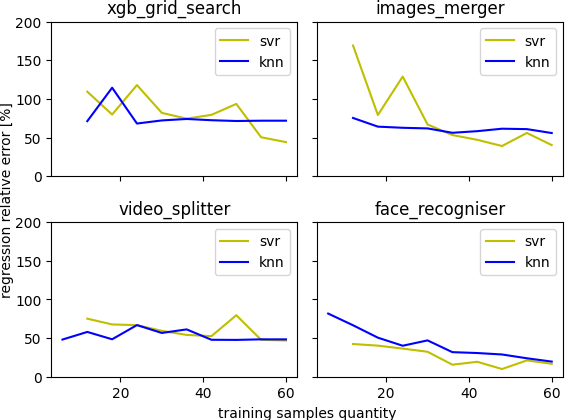
\includegraphics[width=1.0\textwidth]{learning_curve_multi}
	\end{minipage}
	\caption{Learning curve per module.}
	\label{fig:curve}
\end{figure*}

The training pipeline for each module contains the following steps:
\begin{enumerate}
	\item Having the 80 data points, we divide them into training and test data sets with 1:4 proportion.
	\item Standardization of a data set is a common requirement for many machine learning estimators: they might behave badly if the individual features do not more or less look like standard normally distributed data (e.g. Gaussian with 0 mean and unit variance)\cite{scaler}. We scale each column (feature) of the data set using the following formula:
	\[ \vec{x}_{f}^{'} = \frac{\vec{x}_{f}-\mu_f}{\sigma_f} \textnormal{, where:}\]
	\begin{itemize}
		\item $ \vec{x}_{f} $ - data set column \textit{f},
		\item $ \mu_f $ - mean of the column \textit{f},
		\item $ \sigma_f $ - standard deviation of the column \textit{f}.
	\end{itemize}
	\item Each algorithm have a few parameters that should be chosen wisely in order to the better results. It is hard to predict the best value of a continuous parameter. What we did is an exhaustive search over specified parameter values for an estimator from the given possible values. For each combination of the parameter values we validate the model using 5-fold cross validation (as it was mentioned in the first step). It is called a \textit{grid search}\cite{grid_search}.
	\item Finally, we retrained our model using the full data set and the parameters that were found in the previous step.
	\subsection{Support Vector Regression}
	The parameters grid for the \textit{SVR} algorithm is listed below:
	\begin{lstlisting}[language=json,firstnumber=1]
'gamma': [0.0001, 0.0002, 0.0004, 0.0008, 
0.0016, 0.0032, 0.0064, 0.0128], 
'epsilon': [1e-06, 2e-06, 4e-06, 8e-06, 
1.6e-05, 3.2e-05, 6.4e-05, 0.000128, 
0.000256, 0.000512, 0.001024], 
'C': [1000.0, 2000.0, 4000.0, 8000.0,
16000.0, 32000.0, 64000.0, 128000.0, 
256000.0, 512000.0, 1024000.0, 2048000.0]
	\end{lstlisting}
	
	\subsection{K-nearest Neighbors}
	The parameters grid for the \textit{KNN} algorithm is listed below:
	\begin{lstlisting}[language=json,firstnumber=1]
'n_neighbors': [1, 2, 3, 4, 5, 6, 7, 8, 9, 10, 11], 
'weights': ['uniform', 'distance'], 
'p': [1, 2]
	\end{lstlisting}
	
	\begin{figure}[!htb]
		\caption{Visualization of the SVR's epsilon parameter~\citeinside{epsilon}.}
		\centering
		\label{fig:surf_knn_video_splitter}
		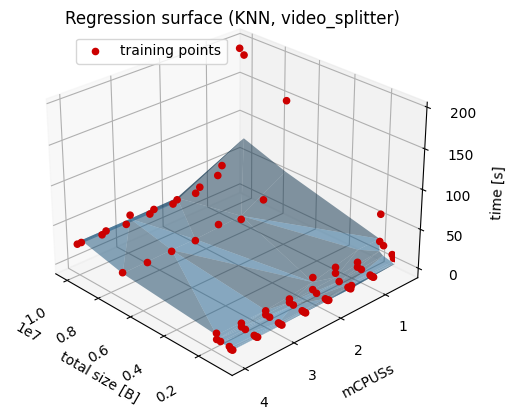
\includegraphics[width=0.49\textwidth]{surf_knn_video_splitter}
	\end{figure}
		
	\subsection{Final results}
	
	\begin{table*}[!t]
		\centering
		\caption{\label{tab:example_df}The results.}
		\begin{minipage}{0.9\linewidth}
			{\footnotesize
				\begin{tabular}{|c c c c >{\columncolor[gray]{0.9}}c|} 
					\hline
					Algorithm & Module name & best params & error [s] & relative error [\%] \\ [0.5ex] 
					\hline\hline
					\textit{SVR} & \textit{Video splitter} & 3131 & 3131 & 3.909 \\ 
					\hline
					\textit{SVR} & \textit{Face recogniser} & 1477 & 1477 & 1.981  \\
					\hline
					\textit{SVR} & \textit{XGB grid search} & 1229 & 1229 & 11.371 \\
					\hline
					\textit{SVR} & \textit{Images merger} & 1229 & 1229 & 11.371 \\ [1ex] 
					\hline
				\end{tabular}
			}
		\end{minipage}
	\end{table*}	
\end{enumerate} 


\subsection{Training}
...
\subsection{Validation}
...